\documentclass[a4paper,11pt,fleqn,twoside,openright ]{memoir} 	% Openright aabner kapitler paa hoejresider (openany begge)

%%%% PACKAGES %%%%

% ¤¤ Oversaettelse og tegnsaetning ¤¤ %
\usepackage[utf8]{inputenc}					% Input-indkodning af tegnsaet (UTF8)
\usepackage[danish]{babel}					% Dokumentets sprog
\usepackage[T1]{fontenc}					% Output-indkodning af tegnsaet (T1)
\usepackage{ragged2e,anyfontsize}			% Justering af elementer
\usepackage{fixltx2e}						% Retter forskellige fejl i LaTeX-kernen
																			
% ¤¤ Figurer og tabeller (floats) ¤¤ %
\usepackage{graphicx} 						% Haandtering af eksterne billeder (JPG, PNG, PDF)
\usepackage{multirow}                		% Fletning af raekker og kolonner (\multicolumn og \multirow)
\usepackage{colortbl} 						% Farver i tabeller (fx \columncolor, \rowcolor og \cellcolor)
\usepackage[dvipsnames]{xcolor}				% Definer farver med \definecolor. Se mere: http://en.wikibooks.org/wiki/LaTeX/Colors
\usepackage{flafter}						% Soerger for at floats ikke optraeder i teksten foer deres reference
\let\newfloat\relax 						% Justering mellem float-pakken og memoir
\usepackage{float}							% Muliggoer eksakt placering af floats, f.eks. \begin{figure}[H]
%\usepackage{eso-pic}						% Tilfoej billedekommandoer paa hver side
%\usepackage{wrapfig}						% Indsaettelse af figurer omsvoebt af tekst. \begin{wrapfigure}{Placering}{Stoerrelse}
%\usepackage{multicol}         	        	% Muliggoer tekst i spalter
%\usepackage{rotating}						% Rotation af tekst med \begin{sideways}...\end{sideways}

% ¤¤ Matematik mm. ¤¤
\usepackage{amsmath,amssymb,stmaryrd} 		% Avancerede matematik-udvidelser
\usepackage{mathtools}						% Andre matematik- og tegnudvidelser
\usepackage{textcomp}                 		% Symbol-udvidelser (f.eks. promille-tegn med \textperthousand )
\usepackage{siunitx}						% Flot og konsistent praesentation af tal og enheder med \si{enhed} og \SI{tal}{enhed}
\sisetup{output-decimal-marker = {,}}		% Opsaetning af \SI (DE for komma som decimalseparator) 
\usepackage[version=3]{mhchem} 				% Kemi-pakke til flot og let notation af formler, f.eks. \ce{Fe2O3}
%\usepackage{rsphrase}						% Kemi-pakke til RS-saetninger, f.eks. \rsphrase{R1}

% ¤¤ Referencer og kilder ¤¤ %
\usepackage[danish]{varioref}				% Muliggoer bl.a. krydshenvisninger med sidetal (\vref)
\usepackage{natbib}							% Udvidelse med naturvidenskabelige citationsmodeller
%\usepackage{xr}							% Referencer til eksternt dokument med \externaldocument{<NAVN>}
%\usepackage{glossaries}					% Terminologi- eller symbolliste (se mere i Daleifs Latex-bog)

% ¤¤ Misc. ¤¤ %
\usepackage{listings}						% Placer kildekode i dokumentet med \begin{lstlisting}...\end{lstlisting}
\usepackage{lipsum}							% Dummy text \lipsum[..]
\usepackage[shortlabels]{enumitem}			% Muliggoer enkelt konfiguration af lister
\usepackage{pdfpages}						% Goer det muligt at inkludere pdf-dokumenter med kommandoen \includepdf[pages={x-y}]{fil.pdf}	
\pdfoptionpdfminorversion=6					% Muliggoer inkludering af pdf dokumenter, af version 1.6 og hoejere
\pretolerance=2500 							% Justering af afstand mellem ord (hoejt tal, mindre orddeling og mere luft mellem ord)

\usepackage{calc}

% Kommentarer og rettelser med \fxnote. Med 'final' i stedet for 'draft' udloeser hver note en error i den faerdige rapport.
\usepackage[footnote,draft,danish,silent,nomargin]{fixme}		


%%%% CUSTOM SETTINGS %%%%

% ¤¤ Marginer ¤¤ %
\setlrmarginsandblock{3.5cm}{2.5cm}{*}		% \setlrmarginsandblock{Indbinding}{Kant}{Ratio}
\setulmarginsandblock{2.5cm}{3.0cm}{*}		% \setulmarginsandblock{Top}{Bund}{Ratio}
\checkandfixthelayout 						% Oversaetter vaerdier til brug for andre pakker

%	¤¤ Afsnitsformatering ¤¤ %
\setlength{\parindent}{0mm}           		% Stoerrelse af indryk
\setlength{\parskip}{3mm}          			% Afstand mellem afsnit ved brug af double Enter
\linespread{1,1}							% Linie afstand

% ¤¤ Litteraturlisten ¤¤ %
\bibpunct[,]{[}{]}{;}{a}{,}{,} 				% Definerer de 6 parametre ved Harvard henvisning (bl.a. parantestype og seperatortegn)
\bibliographystyle{bibtex/harvard}			% Udseende af litteraturlisten.

% ¤¤ Indholdsfortegnelse ¤¤ %
\setsecnumdepth{subsection}		 			% Dybden af nummerede overkrifter (part/chapter/section/subsection)
\maxsecnumdepth{subsection}					% Dokumentklassens graense for nummereringsdybde
\settocdepth{subsection} 					% Dybden af indholdsfortegnelsen

% ¤¤ Lister ¤¤ %
\setlist{
  topsep=0pt,								% Vertikal afstand mellem tekst og listen
  itemsep=-1ex,								% Vertikal afstand mellem items
} 

% ¤¤ Visuelle referencer ¤¤ %
\usepackage[colorlinks]{hyperref}			% Danner klikbare referencer (hyperlinks) i dokumentet.
\hypersetup{colorlinks = true,				% Opsaetning af farvede hyperlinks (interne links, citeringer og URL)
    linkcolor = black,
    citecolor = black,
    urlcolor = black
}

% ¤¤ Opsaetning af figur- og tabeltekst ¤¤ %
\captionnamefont{\small\bfseries\itshape}	% Opsaetning af tekstdelen ('Figur' eller 'Tabel')
\captiontitlefont{\small}					% Opsaetning af nummerering
\captiondelim{. }							% Seperator mellem nummerering og figurtekst
\hangcaption								% Venstrejusterer flere-liniers figurtekst under hinanden
\captionwidth{\linewidth}					% Bredden af figurteksten
\setlength{\belowcaptionskip}{0pt}			% Afstand under figurteksten
		
% ¤¤ Opsaetning af listings ¤¤ %
\definecolor{commentGreen}{RGB}{34,139,24}
\definecolor{stringPurple}{RGB}{208,76,239}

\lstset{language=Matlab,					% Sprog
	basicstyle=\ttfamily\scriptsize,		% Opsaetning af teksten
	keywords={for,if,while,else,elseif,		% Noegleord at fremhaeve
			  end,break,return,case,
			  switch,function},
	keywordstyle=\color{blue},				% Opsaetning af noegleord
	commentstyle=\color{commentGreen},		% Opsaetning af kommentarer
	stringstyle=\color{stringPurple},		% Opsaetning af strenge
	showstringspaces=false,					% Mellemrum i strenge enten vist eller blanke
	numbers=left, numberstyle=\tiny,		% Linjenumre
	extendedchars=true, 					% Tillader specielle karakterer
	columns=flexible,						% Kolonnejustering
	breaklines, breakatwhitespace=true,		% Bryd lange linjer
}

% ¤¤ Navngivning ¤¤ %
\addto\captionsdanish{
	\renewcommand\appendixname{Appendiks}
	\renewcommand\contentsname{Indholdsfortegnelse}	
	\renewcommand\appendixpagename{Appendiks}
	\renewcommand\appendixtocname{Appendiks}
	\renewcommand\cftchaptername{\chaptername~}				% Skriver "Kapitel" foran kapitlerne i indholdsfortegnelsen
	\renewcommand\cftappendixname{\appendixname~}			% Skriver "Appendiks" foran appendiks i indholdsfortegnelsen
}

% ¤¤ Kapiteludssende ¤¤ %

\newif\ifNoChapNumber
\makeatletter
\makechapterstyle{VZ34}{
	\renewcommand\chapternamenum{}
	\renewcommand\printchaptername{}
	\renewcommand\printchapternum{}
	\renewcommand\chapnumfont{\Huge\bfseries}
	\renewcommand\chaptitlefont{\Huge\bfseries\raggedright}
	\renewcommand\printchaptertitle[1]{%
		\begin{tabular}{@{}p{1cm}|!{\quad}p{\textwidth-1cm-2em-4\tabcolsep }}
			\ifNoChapNumber\relax\else\chapnumfont \thechapter\fi
			& \chaptitlefont ##1
		\end{tabular}
		\NoChapNumberfalse
	}
	\renewcommand\printchapternonum{\NoChapNumbertrue}
}
\chapterstyle{VZ34}

% ¤¤ Sidehoved ¤¤ %

\makepagestyle{Uni}							% Definerer sidehoved og sidefod udseende frem til ...
\makepsmarks{Uni}{%
	\createmark{chapter}{left}{shownumber}{}{. \ }
	\createmark{section}{right}{shownumber}{}{. \ }
	\createplainmark{toc}{both}{\contentsname}
	\createplainmark{lof}{both}{\listfigurename}
	\createplainmark{lot}{both}{\listtablename}
	\createplainmark{bib}{both}{\bibname}
	\createplainmark{index}{both}{\indexname}
	\createplainmark{glossary}{both}{\glossaryname}
}
\nouppercaseheads											% Ingen Caps oenskes

\makeevenhead{Uni}{Gruppe B131}{}{\leftmark}				% Definerer lige siders sidehoved (\makeevenhead{Navn}{Venstre}{Center}{Hoejre})
\makeoddhead{Uni}{\rightmark}{}{Dit Universitet}			% Definerer ulige siders sidehoved (\makeoddhead{Navn}{Venstre}{Center}{Hoejre})
\makeevenfoot{Uni}{\thepage}{}{}							% Definerer lige siders sidefod (\makeevenfoot{Navn}{Venstre}{Center}{Hoejre})
\makeoddfoot{Uni}{}{}{\thepage}								% Definerer ulige siders sidefod (\makeoddfoot{Navn}{Venstre}{Center}{Hoejre})
\makeheadrule{Uni}{\textwidth}{0.5pt}						% Tilfoejer en streg under sidehovedets indhold
\makefootrule{Uni}{\textwidth}{0.5pt}{1mm}					% Tilfoejer en streg under sidefodens indhold

\copypagestyle{Unichap}{Uni}								% Sidehoved for kapitelsider defineres som standardsider, men med blank sidehoved
\makeoddhead{Unichap}{}{}{}
\makeevenhead{Unichap}{}{}{}
\makeheadrule{Unichap}{\textwidth}{0pt}
\aliaspagestyle{chapter}{Unichap}							% Den ny style vaelges til at gaelde for chapters
															% ... her
															
\pagestyle{Uni}												% Valg af sidehoved og sidefod (benyt "plain" for ingen sidehoved/fod)


%%%% CUSTOM COMMANDS %%%%

% ¤¤ Billede hack ¤¤ %										% Indsaet figurer nemt med \figur{Stoerrelse}{Fil}{Figurtekst}{Label}
\newcommand{\figur}[4]{
		\begin{figure}[H] \centering
			\includegraphics[width=#1\textwidth]{billeder/#2}
			\caption{#3}\label{#4}
		\end{figure} 
}

% ¤¤ Specielle tegn ¤¤ %
\newcommand{\decC}{^{\circ}\text{C}}
\newcommand{\dec}{^{\circ}}
\newcommand{\m}{\cdot}


%%%% ORDDELING %%%%

\hyphenation{}											% Preamble indlaeses
\raggedbottom													% Soerger for at LaTeX ikke "straekker" teksten

%\includeonly{file1,file2}										% Inkluder kun specifikke filer (kommasepareret liste)

\begin{document}												% Starter dokumentet - obligatorisk


\frontmatter													% Forindhold - nummereres med romertal

\thispagestyle{empty} % Remove page numbering on this page


\colorbox{usDef}{
	\parbox[t]{1.0\linewidth}{
		\centering \fontsize{30pt}{50pt}\selectfont % The first argument for fontsize is the font size of the text and the second is the line spacing - you may need to play with these for your particular title
		\vspace*{0.7cm} % Space between the start of the title and the top of the grey box
		
		\hfill Remote Ischemic Conditioning\\
		\hfill Udviklingsdokumentation \\
		
		\vspace*{0.7cm} % Space between the end of the title and the bottom of the grey box
	}
}

\vfill % Space between the title box and author information


{\centering \large 
	\hfill Simon Vammen Grønbæk \\
	\hfill Karl-Johan Schmidt\\
	\hfill Aarhus University \\
	\hfill Aarhus School of Engineering\\
	\hfill Efteråret 2015 \\
}

\clearpage % Whitespace to the end of the page
\cleardoublepage												% Indsaetter tom side, saa naeste kapitel starter paa hoejre side (hvis noedvendigt)
% Dette er et titelblad designet til videregående uddannelser på et universitet
% Filen kræver:
% Universitetets logo:  AU-logo-DK eller AU-logo-DK
% Synopsis: En fil ved navn synopsis.tex

% Udarbejdet af: Jesper Nørgaard (jesper@noergaard.eu) 10. april 2012

\phantomsection
\pdfbookmark[0]{Titelblad}{titelblad}
\thispagestyle{empty}

\begin{minipage}[t]{0.48\textwidth}
\vspace*{-8pt}			

\includegraphics[height=2.5cm]{billeder/AU-logo-DK}
\end{minipage}
\hfill
\begin{minipage}[t]{0.48\textwidth}
{\small 
\textbf{Ingeniørhøjskolen Aarhus}\\
Finlandsgade 22 \\
8200 Aarhus N \\
Tlf: 8715 0000 \\
http://www.ase.au.dk/}
\end{minipage}

\vspace*{1cm}

\begin{minipage}[t]{0.48\textwidth}
\textbf{Titel:} \\[5pt]\bigskip\hspace{2ex}
Remote Ischemic Conditioning

\textbf{Projekt:} \\[5pt]\bigskip\hspace{2ex}
Bachelor projekt

\textbf{Projektperiode:} \\[5pt]\bigskip\hspace{2ex}
Juli 2015 - December 2015

\textbf{Projektgruppe:} \\[5pt]\bigskip\hspace{2ex}
15155

\textbf{Deltagere:} \\[5pt]\hspace*{2ex}
Simon Vammen Grønbæk\\\hspace*{2ex}
Karl-Johan Schmidt \\\hspace*{2ex}


\textbf{Vejledere:} \\[5pt]\hspace*{2ex}
Peter Johansen \\\bigskip\hspace{2ex}

\textbf{Projektudbyder:} \\[5pt]\hspace*{2ex}
Rolf Blauenfeldt\\\bigskip\hspace{2ex}
\vspace*{4cm}

\textbf{Oplagstal: 10} \\
\textbf{Sidetal: \pageref{SidsteSide}} \\
\textbf{Afsluttet 18-12-2014}

\end{minipage}
\hfill
\begin{minipage}[t]{0.483\textwidth}
	\textbf{Godkendelse:}\vspace{1cm}
\begin{table}[H]
	\centering
	\begin{tabular}{c}
		\underline{\phantom{mmmmmmmmmmmmmm}}  \\
		Karl-Johan Schmidt \vspace{2cm}\\
		\underline{\phantom{mmmmmmmmmmmmmm}} \\
		Simon Vammen Grønbæk \vspace{2cm}	\\
		\underline{\phantom{mmmmmmmmmmmmmm}} \\
		Peter Johansen \vspace{2cm}	\\
		\underline{\phantom{mmmmmmmmmmmmmm}} \\
		Rolf Blauenfeldt \vspace{2cm}	\\
	\end{tabular}
\end{table}
\end{minipage}

\vfill

{\footnotesize\itshape Rapportens indhold er frit tilgængeligt, men offentliggørelse (med kildeangivelse) må kun ske efter aftale med forfatterne.}

% Rapportens indhold er frit tilgængeligt, men offentliggørelse (med kildeangivelse) må kun ske efter aftale med forfatterne.
% The content of the report is freely available, but publication (with source reference) may only take place in agreement with the authors.

\cleardoublepage
\chapter*{Forord}

\textit{Indsæt forord}

\textbf{Læsevejledning}

Der vil igennem rapporten fremtræde kildehenvisninger, og disse vil være samlet i en kildeliste bagerst i rapporten. Der er i rapporten anvendt kildehenvisning efter Harvardmetoden, så i teksten refereres en kilde med [Efternavn, År]. Denne henvisning fører til kildelisten, hvor bøger er angivet med forfatter, titel, udgave og forlag, mens Internetsider er angivet med forfatter, titel og dato. Figurer og tabeller er nummereret i henhold til kapitel, dvs. den første figur i kapitel 7 har nummer 7.1, den anden, nummer 7.2 osv. Forklarende tekst til figurer og tabeller findes under de givne figurer og tabeller.


\vspace{3cm}
\begin{table}[H]
	\centering
		\begin{tabular}{c c}
			\underline{\phantom{mmmmmmmmmmmmmm}} & \underline{\phantom{mmmmmmmmmmmmmm}} \\
			Karl-Johan Schmidt	& Simon Vammen Grønbæk	\\
		\end{tabular}
\end{table}
\cleardoublepage

%%%% Indholdsfortegnelse (TOC) %%%%

\phantomsection													% Kunstigt afsnit, som hyperlinks kan 'holde fast i'
\pdfbookmark[0]{Indholdsfortegnelse}{indhold}					% Tildeler en klikbar bookmark til den endelige PDF
\tableofcontents*												% Indholdsfortegnelsen (kaldet ToC) 

%\addtocontents{toc}{\protect\newpage}							% Fremtvinger sideskift i ToC hvis noedvendig (der hvor koden placeres)


\mainmatter														% Hovedindhold - nummereres fra side 1

%%%% Rapportindhold %%%% 										% Rapportindholdet boer IKKE indeholde broedtekst - KUN includede filer!

%% Indledende %%												% Opdel evt. i passende afsnit for overblikkets skyld

\chapter{Indledning}
Neurologisk afdeling på Aarhus Universitetshospital skal i et kommende studie undersøge effekten af \textit{Remote Ischemic Pre- og Postcondtioning}. \textit{Remote ischemic conditiong (RIC)} er en behandlingsform, som har vist lovende resultater i forebyggelse og behandling af patienter med blodprop i hjertet. Studiet ønsker at undersøge, om denne behandlingsform kan have samme gavnlige effekt på patienter med apopleksi. For at studiet skal kunne gennemføres, har afdelingen kontaktet Ingeniørhøjskolen, Aarhus Universitet, omkring udvikling af det apparat, som skal udføre RIC behandlingen under studiet. Denne udviklingsopgave blev til dette bachelorprojekt. 

\section{Formål}
Formålet med denne projektrapport er at beskrive projektforløbet i forbindelse med udviklingen af \textit{Konditioneringsapparatet}. Rapporten beskriver den faglige baggrund for projektet og behovet for et modificeret blodtryksapparat (konditioneringsapparat). Hernæst gennemgås hvilke afgrænsninger, projektgruppen har foretaget. Ydermere er formålet med rapporten at sikre, læseren har en forståelse for, hvilke metoder der er anvendt i projektforløbet samt resultatet og diskussion af den opnåede prototype. 

\section{Læsevejledning}
Projektrapporten skal læses som resultatet af projektforløbet. Rapporten er opdelt i følgende kapitler;

	\begin{longtable}{ p{0.14\textwidth} p{0.8\textwidth} } 
		Kapitel 1 & Præsentation af indledende punkter omkring bachelorprojektet, \textit{Remote ischemic conditioning}\\
		Kapitel 2 & Her beskrives den viden, der ligger til grund for forståelsen af projektet. \\
		Kapitel 3 & Beskrivelse af problemformuleringen, som er udarbejdet i samarbejde med kunden og vejlederen\\
		Kapitel 4 & Præsentation af områder, hvor projektet er blevet afgrænset\\
		Kapitel 5 & Giver en kort beskrivelse af den udviklede prototype\\
		Kapitel 6 & Redegørelse for hvilke ingeniørfaglige metoder projektet har gjort brug af \\
		Kapitel 7 & Præsentation af de centrale opnåede resultater ved produktudviklingen og projektforløbet\\
		Kapitel 8 & Beskrivelse og gennemgang af diskussionspunkter omkring de centrale resultater\\
		Kapitel 9 & Redegørelse for fremtiden for prototypen\\ 
		Kapitel 10& Indeholder en opsamling og konklusion på projektforløbet og prototypen\\
	\end{longtable}

\subsubsection{Appendiks}
Appendiksafsnittet indeholder logbog, tidsplan, samarbejdsaftale mm. Dette afsnit skal læses som dokumentation for projektforløbet

\subsubsection{Udviklingsdokumentation}
Foruden projektsrapporten består projektgruppens skriftlige produkt også af et udviklingsdokument. Dette udviklingsdokument giver læseren fuldt indblik i udviklingsfasen af \textit{Konditioneringsapparatet}. Dokument består af 4 underdokumenter, hhv. kravspecifikation, accepttest, system design og implementering. 

Dokumentationsrapporten bygger på udviklingsdokumentationen, som af denne grund er fungerende som opslagsdokument for dokumentationsrapporten. Se udviklingsdokumentet i vedlagte ZIP-fil under \textit{Konditioneringsapparat/udviklingsdokument.pdf}.




\chapter{Projektbeskrivelse}

Projektforslaget lægger op til at belyse effekterne af energirenovering samt hvordan barrierne overvindes ved brug af virkemidler. 

I det følgende reflekteres der over emnerne i problemanalysen. Problemformuleringen indrammer herefter projektet inden det konkretiseres i afgrænsningen. Endelig beskrives de metoder, som søges anvendt. 

\section{Problemanalyse}

\section{Problemformulering}

I den kontekstuelle del søges følgende spørgsmål besvaret.

I den tekniske del søges følgende energi- og konstruktionsmæssige spørgsmål besvaret.

\section{Projektafgrænsning}

\section{Metode}

%% Kontekst %%

\chapter{Baggrund}


\chapter{Screening af virkemidler}

På trods af at der renoveres meget af den eksisterende bygningsmasse, så kniber det ofte med at få foretaget oplagte energirenoveringer i samme ombæring. I det følgende vil der blive foretaget en screening af potentielle virkemidler, som kan fremme energirenovering og energieffektivisering i øvrigt. I fokus er:

\begin{itemize}
\item Økonomi/tilskud
\item Lovgivning
\item Informationsindsats
\item Individuel måling
\end{itemize}

De tre første punkter er universelle virkemidler, men perspektiveres til energirenovering. Det sidste punkt relaterer sig til energieffektivisering i en bredere kontekst. Det betragtes dog stadig som et virkemiddel, idet det er beviseligt, at overgang fra kollektiv til individuel afregning af forbrugsposter (el, vand og varme) medfører energibesparelser \citep{maalere}.

%% Teknisk %%

\chapter{Energiberegning} \label{sec:energi}

Med henblik på at beregne rentabiliteten af de valgte energirenoveringstiltag, må den forventede besparelse kortlægges. Det gøres ved at betragte bygningens energiforbrug før og efter forbedringen. Hertil benyttes graddøgnsmetoden.

\section{Graddøgnsmetoden}

Graddage er et gammelt udtryk for et varmebehov angivet i enheden "grader gange dage". Det er således forskellen mellem en korrigeret indetemperatur og udetemperatur, ganget med en periode hvori temperaturforskellen har optrådt. Den korrigerede indetemperatur er lavere end rumtemperatur, idet der udnyttes et varmetilskud fra solindfald, personer og udstyr. Bygningens varmeanlæg skal således varme op til denne basistemperatur, som den kaldes. Graddagstal er baseret på basistemperaturen 17 $\decC$. Princippet er illustreret på figur \ref{fig:gdmetode}.

\begin{figure}[H]
	\centering
	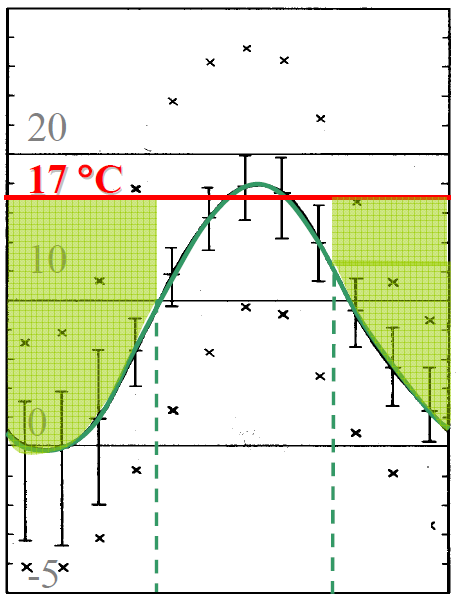
\includegraphics[width=0.55\textwidth]{billeder/graddage.png}
	\caption{Graddagene er illustreret som forskellen mellem basistemperaturen og udetemperaturen (i opvarmningssæsonen angivet med stiplede linjer) og er markeret med grønt.}
	\label{fig:gdmetode}
\end{figure}

Antallet af graddage årligt i Danmark er ca. 3.000. Når bygningsdelenes termiske egenskaber kendes, kan det forventede årlige energiforbrug, $E$, beregnes med ligning \eqref{eq:GD}. De anvendte forudsætninger kan findes i beskrivelsen af casehuset i appendiks \ref{sec:casehus}.

\begin{align}		
E = B_u \m 24 \m G			
\label{eq:GD} 
\end{align}

% \m er i preamble kodet til at gælde som \cdot (gangeprik) for at lette arbejdet

Hvor:
\begin{table}[H]
\begin{tabular}{l|l}
	$E$					& Det forventede energiforbrug [\si{Wh/\text{å}r}] \\
	$B_u$ 				& Bygningens specifikke varmetab ved transmission og ventilation [\si{W/K}] \\
	$24$ 				& Døgnets timer [\si{h/d\text{ø}gn}] \\
	$G$					& Graddage [\si{K d\text{ø}gn/\text{å}r}]
\end{tabular}
\end{table}

Bygningens specifikke varmetab består af bidrag fra transmissionstab og ventilationstab.\fxnote{Skriv færdigt i morgen}


\chapter{Stålmateriale}

Inden der kan regnes på en stålkonstruktion, der skal opsættes i forbindelse med en gennemgribende renovering, beskrives stålet som materiale.

\section{Fremstilling}

\section{Egenskaber}

\fxnote{Husk at skrive om egenskaber ved brand, Jens!}

\subsection{Arbejdskurve}

Den nederste del af ståls arbejdskurve følger principperne om Hook's lov \citep[ s. 419]{fysikbog}.

%% Afrunding %%

\chapter{Konklusion}

I kapitel \ref{sec:energi} blev den energirenoverede bygnings forventede energibesparelse udregnet.


%%%% Kilder %%%%

\begingroup
	\raggedright
	\bibliography{bibtex/litteratur}							% Litteraturlisten inkluderes
\endgroup


%%%% Fixme-listen %%%%

\newpage														% Ny side til Fixme-listen
\listoffixmes													% Fixme-listen - fjernes til sidst i projektet med "%"


%%%% Appendiks %%%%

\appendix														% Appendiks/bilag start - giver chapter bogstaver i stedet for tal
\clearforchapter												% Sikrer at pagestylen aktiveres paa den rigtige side
\phantomsection													% Kunstigt afsnit, som hyperlinks kan 'holde fast i'
\pdfbookmark[0]{Appendiks}{appendiks}							% Tildeler en klikbar bookmark til den endelige PDF

%% Indstillinger for appendiks (deaktiveret med "%") %%

%\pagestyle{empty}												% Sidehoved/-fod for standardsider aendres til tom for appendiks
%\aliaspagestyle{chapter}{empty}								% Sidehoved/-fod for kapitelsider aendres til tom for appendiks
%\settocdepth{chapter}											% Kun kapitel-niveau vises i ToC
%\addtocontents{toc}{\protect\cftpagenumbersoff{chapter}}		% Sidetal for kapitler fjernes i ToC

%% Filer til appendiks %%

\chapter{Appendiks} 


\section{Test med pulsoximeter} \label{app:pulstest}

Test resultater ved aklemning af arm ved 220 mmHg sammenholdt med pulsoximeter
\begin{longtable}{p{0.14\textwidth} p{0.14\textwidth} p{0.14\textwidth} p{0.14\textwidth} }
	\hline
	Tid [s] & Saturation [\%] & Puls [bpm] & Tryk [mmHg] \\ \hline
	0 &	100 &	54 &	0 \\ \hline
	30 &	100 &	48 &	220 \\ \hline
	60 &	100 &	41 &	220 \\ \hline
	90 &	100	& 45  &	220 \\ \hline
	120	& 0	& 0	& 220 \\ \hline
	150 &	100 &	52 &	220 \\ \hline
	180	& 0 &	0 &	220 \\ \hline
	210	& 0	 & 0 &	220 \\ \hline
	240 &	0 &	0 &	220 \\ \hline
	270 &	0 &	0 &	220 \\ \hline
	300 &	0 &	0 &	220 \\ \hline
	310 &	91 &	64 &	0 \\ \hline
	320 &	100 &	60 &	0 \\ \hline
	330 &	100 &	57 &	0 \\ \hline
	600 &	98 &	56 &	0 \\ \hline
	630 &	100 &	52 &	220 \\ \hline
	660 &	100 &	52 &	220 \\ \hline
	690 &	100 &	46 &	220 \\ \hline
	720 &	100 &	50 &	220 \\ \hline
	750	 & 100 &	42 &	220 \\ \hline
	780 &	0 &	0 &	220 \\ \hline
	810 &	0 &	0 &	220 \\ \hline
	840 &	0 &	0 &	220 \\ \hline
	870 &	0 &	0 &	220 \\ \hline
	900 &	0 &	0 &	220 \\ \hline
	910 &	0 &	0 &	0 \\ \hline
	920 &	100 &	61 &	0 \\ \hline
	920 &	96 &	60 &	0 \\ \hline
\end{longtable}
\newpage
\section{Samarbejdsaftale - intern}\label{title:samarbejdsaftaleIntern}

\textbf{Faglige forventninger til projektet:}
\begin{itemize}
	\item Vi forventer at udarbejde et projekt, som vi kan stå inde for
	\item Vi forventer at det faglige niveau lever op til kravene i kursus beskrivelsen
	\item Vi forventer at der gøre brug af viden og kompetencer fra tidligere kursuser
	\item Vi forventer at gruppens medlemmer viser engagement i projektet
	\item Det forventes at projektet lever op til en topkarakter
\end{itemize}

\textbf{Forventninger til gruppearbejdet og interne aftale:}
\begin{itemize}
	\item Alle gruppemedlemmer deltager aktivt og yder efter bedste evne
	\item Bidrager til konstruktivt diskussioner og problemstillinger undervejs i projektforløbet
	\item Alle aftaler indskrives i den fælles Google Calender, hvor det er eget ansvar at være opdateret
	\item Alle dokumenter der ikke kræver versionshistorik gemmes i gruppens fælles Dropbox mappe
	\item Versionsstyring af dokumenter foregår i git, og det er eget ansvar at ajourføre sine ændringer
	\item Eget ansvar at give besked til gruppen hvis man bliver forhindret i at møde til den ellers aftalte tid
	\item Der må forventes at gruppemedlemmerne pålægges hjemme opgaver og det er eget ansvar at løse disse
	\item Den forventede mødetid i hverdage er 8.15 til 16
	\item Det er et fælles ansvar at oprette en ugentlig plan for ugens opgaver, samt føre logbog over den forgangne uge	
	\item Vi forventer et vejledermøde hver anden uge
	\item Gruppens medlemmer overholder de ovenstående aftale
\end{itemize}

\hspace{3cm}

Underskrives af: 




\begin{table}[H]
	\centering
	\begin{tabular}{c c}
		\underline{\phantom{mmmmmmmmmmmmmmmmmmmmm}} & \underline{\phantom{mmmmmmmmmmmmmmmmmmmmm}} \\
		Simon Vammen Grønbæk (201270788) \vspace{2cm} & Karl-Johan Schmidt (201270751) \vspace{2cm}\\
	\end{tabular}
\end{table}

\newpage
\section{Samarbejdsaftale - reviewgruppe}\label{title:samarbejdsaftaleReview}

Forventninger til samarbejdet:
\begin{itemize}
	\item For hver milepæl i projektet udføres reviewmøder
	\item Efter hvert endt reviewmøde aftales et ny dato for næste møde
	\item De aftalte deadlines forventes overholdt
	\item Vi forventer at reviewgruppen kommer med kontruktiv kritik af det udleverede materiale
	\item Der forventes at grupperne har diskuteret materialet intern, inden det aftalte reviewmøde
	\item Vi forventer at reviewsamarbejdet styrker projekts fremgang og bidrager til et veludarbejdet projekt
	\item Der forventes som minimum to dage fra materiale udleveres til review, før det kan gennemgås. 
\end{itemize}

\hspace{3cm}

Projektgruppens underskrift: 
\begin{table}[H]
	\centering
	\begin{tabular}{c c}
		\underline{\phantom{mmmmmmmmmmmmmmmmmmmmm}} & \underline{\phantom{mmmmmmmmmmmmmmmmmmmmm}} \\
		Simon Vammen Grønbæk (201270788) \vspace{2cm} & Karl-Johan Schmidt (201270751) \vspace{2cm}\\
	\end{tabular}
\end{table}
Reviewgruppens underskrift:
\begin{table}[H]
	\centering
	\begin{tabular}{c c}
		\underline{\phantom{mmmmmmmmmmmmmmmmmmmmm}} & \underline{\phantom{mmmmmmmmmmmmmmmmmmmmm}} \\
		Anders Toft (11242) \vspace{2cm} & Anders Esager (201270874) \vspace{2cm}\\
	\end{tabular}
\end{table}

\newpage

\section{Tidsplan}\label{title:tidsplan}
\begin{figure}[H]
	\centering
	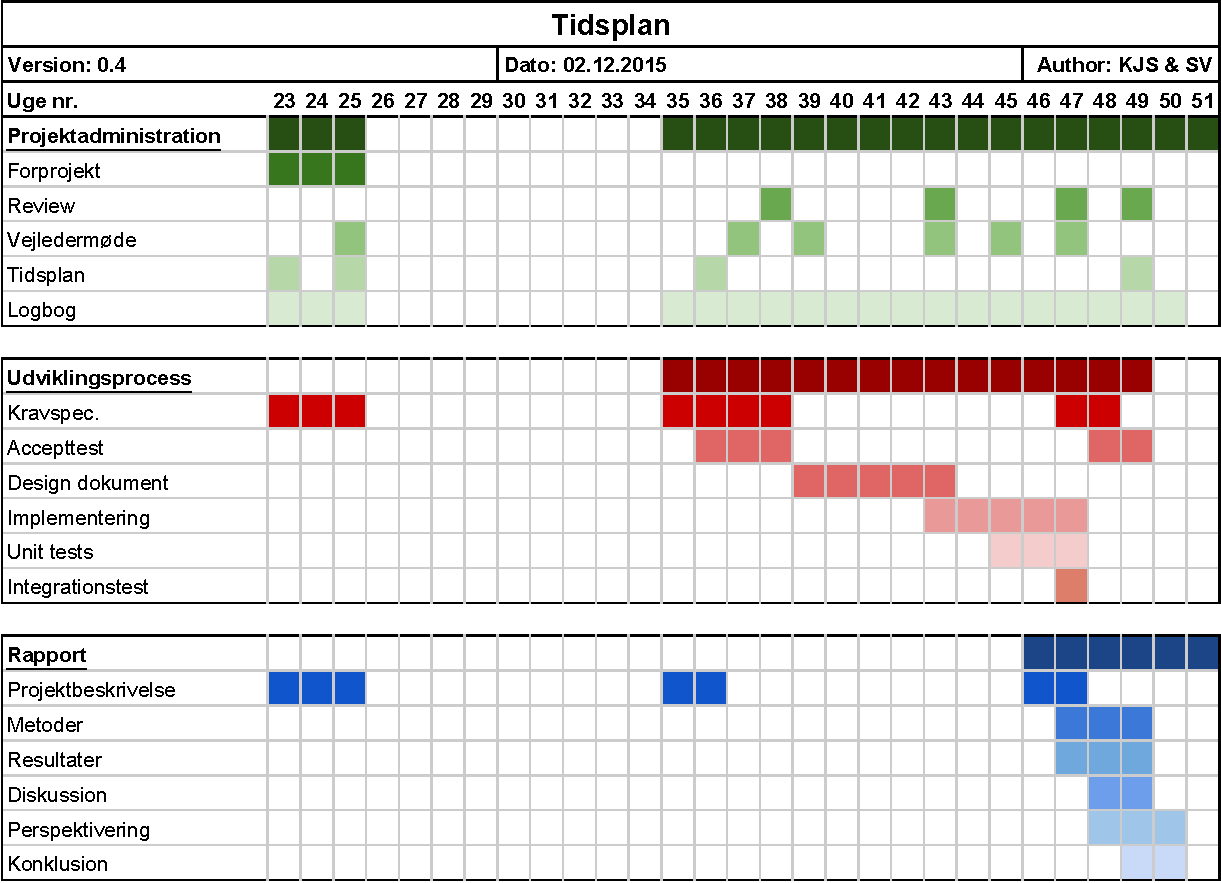
\includegraphics[width = 1.3\textwidth, angle=90,origin=c]{billeder/Tidsplanv04.pdf}
	\caption{Gantt chart over projektforløb}
\end{figure}

\newpage
\section{Fortrolighedsaftale - reviewgruppe} \label{app:tavshedserkl}
\begin{figure}[H]
	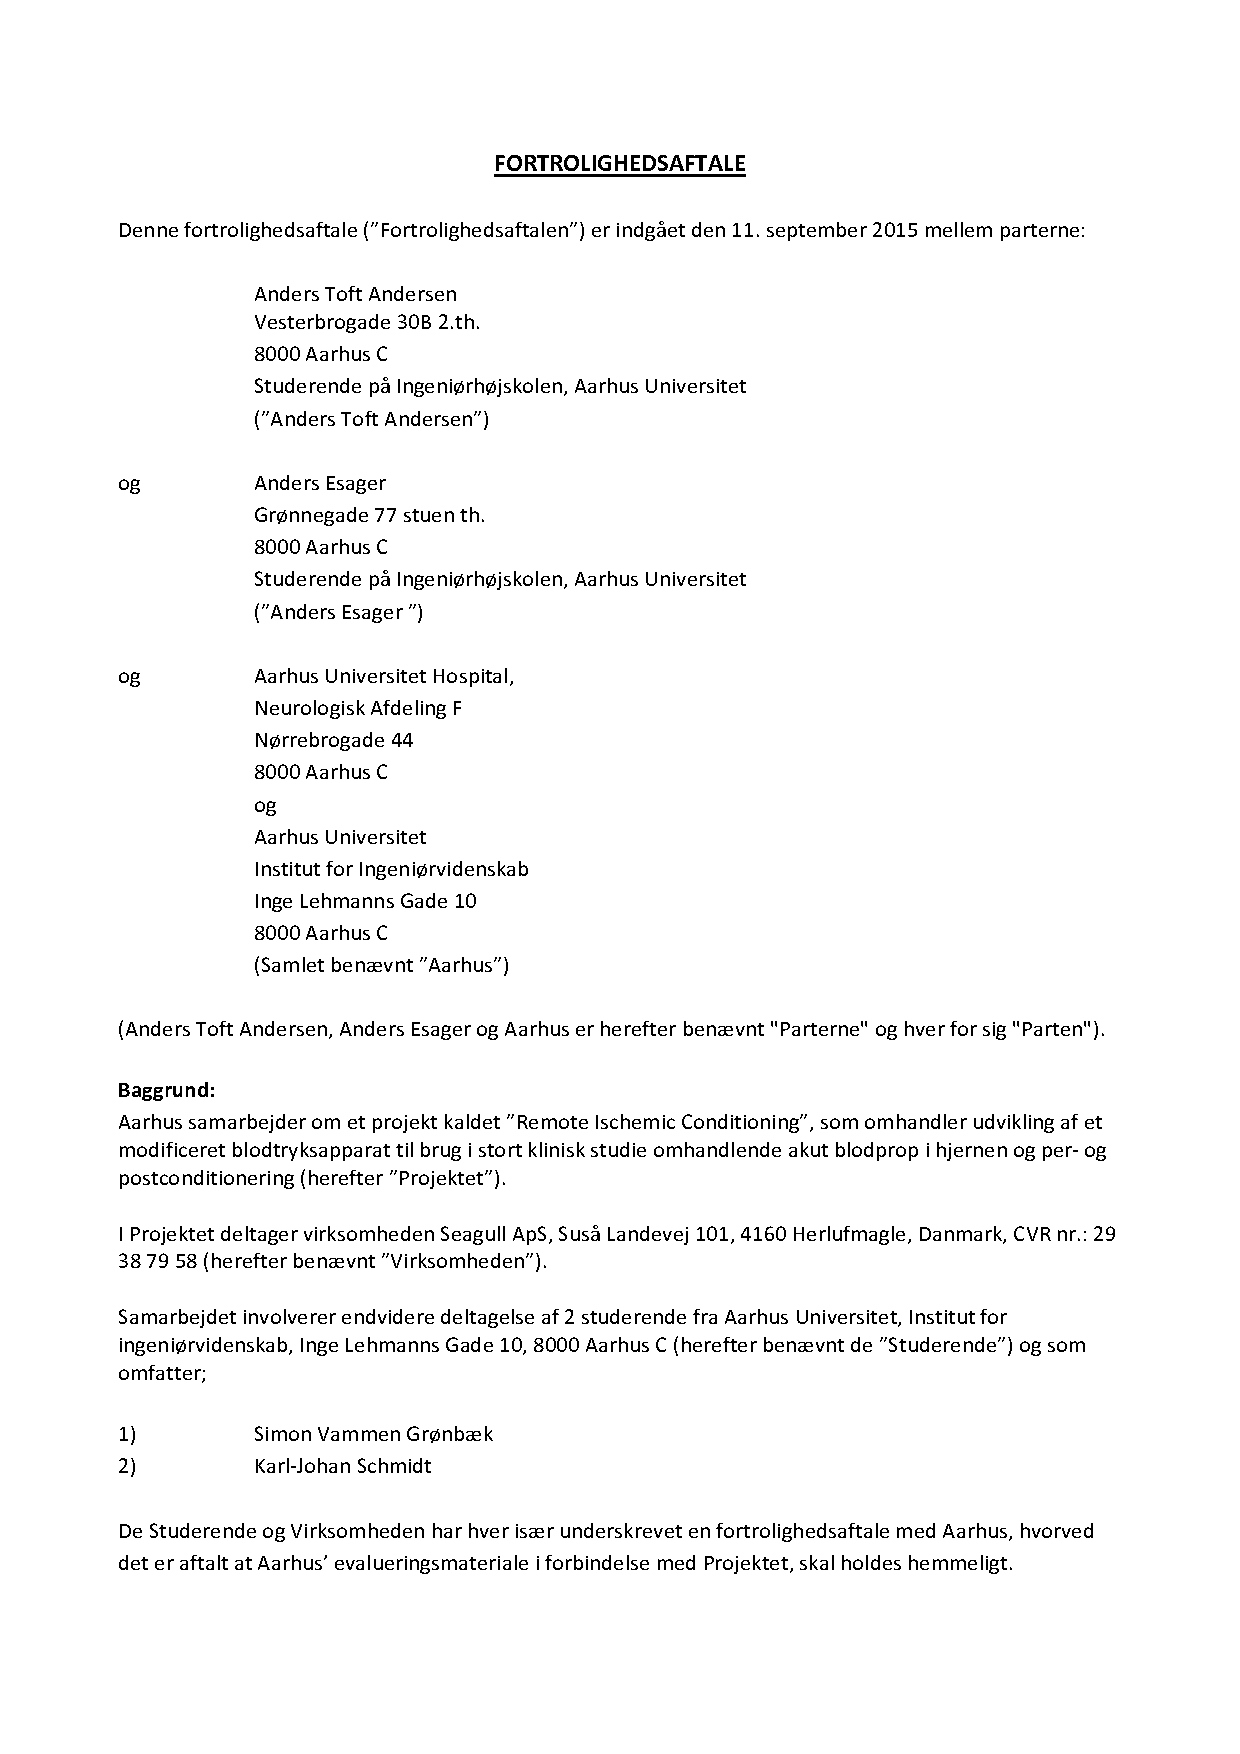
\includegraphics[width = 1\textwidth]{billeder/FortrolighedsaftaleSide1.pdf}
\end{figure}
\newpage
\begin{figure}[H]
	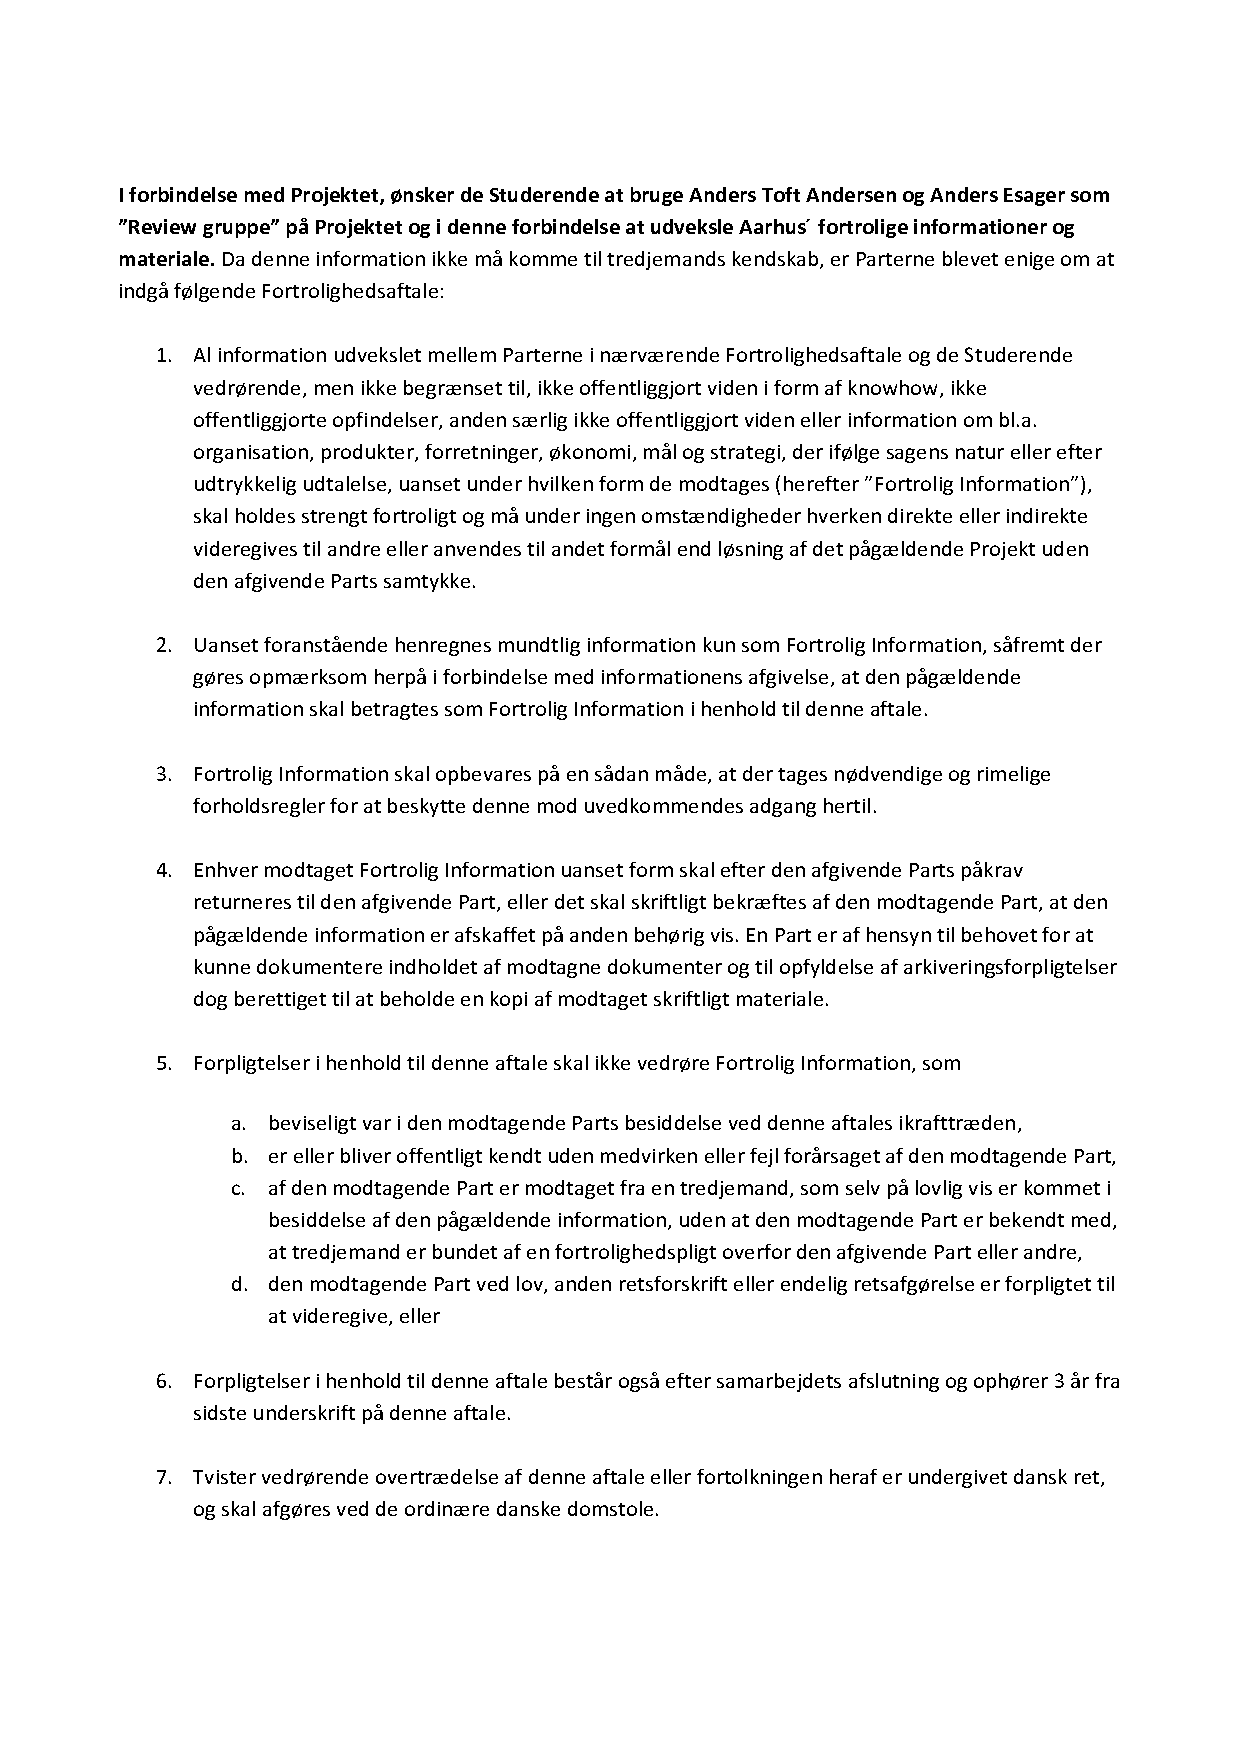
\includegraphics[width = 1\textwidth]{billeder/FortrolighedsaftaleSide2.pdf}
\end{figure}
\newpage
\begin{figure}[H]
	
\includegraphics[width = 1\textwidth]{billeder/FortrolighedsaftaleSide3.pdf}
\end{figure}
\newpage
\section{Kalibrering af blodtrykmåler}
Test på medicoteknisk værksted d. 13/11
Tilstede: KJS og SVG
Den 13/11 var vi på medicoteknisk værksted for at teste prototypen på et blodtryksimulator. Undervej opstod der en række problemer

Prototype systemet er udstyret med en ventil, som hver gang der detekteres en puls åbner og lukker luft ud. Det viste sig at ventilen forstyrede signal og gjorde det umuligt at detektere nogle peaks fra blodtryksimulatoren. Det lykkes at lave blodtrykmåling ved at lave en lille utæthed i system og på den måde sikre at luften slipper ud. 

Simulator: 
Fluke biomedical BP pump2
\url{http://www.maquet-dynamed.com/inside_sales/literature/fluke/bp_\%20pump_2_datasheet.pdf}

Dog var peak’ene stadig mindre end når vi målte på os selv. 

\begin{enumerate}
	\item Første måling med udtæthed: 
	115 sys, 111 map ud fra simulation på 120/80 (93)
	142 sys, 138 map ud fra simulation på 150/100 (116)
	
	\item Vi ændrede på offsetet fra sensoren fra 79 til 88 så nu hedder formlen fra rå værdi til tryk: 
	tryk = (råværdi - 88 ) * 0.408
	
	\item Efter ændring af omregning fra råværdi til mmhg 
	128 sys, 124 map ud fra simulation på 150/100 (116), filnavn “newOffset1.txt” 
	
	\item Ændret alpha til = 0.13 og systole peak at 0.6
	132 sys, 118 map ud fra simulation på 150/100 (116), filnavn “newOffset2.txt” 
	
	\item Jo større utæt vi “laver” i systemet, jo senere kommer amplituderne og jo sværere bliver det at detektere systolisk tryk
	
	\item Ændret threshold = 25
	110 sys, 95 map ud fra simulation på 120/80 (93), filnavn “newOffset3.txt” 
	Denne måling gav et forhold mellem sys og map på 0,31. 
	
	\item SYS/MAP = 0.31, DIA/MAP = 0.51 
	\begin{enumerate}
		\item 120 sys, 95 map, 80 dia ud fra simulation på 120/80 (93), filnavn “newOffset4.txt” 
		\item 149 sys, 119 map, 100 dia ud fra simulation på 150/100 (116), filnavn “newOffset5.txt” 
		\item 129 sys 83 map, 52 dia ud fra omrom apparat på 128/61(84), filnavn “KJ1.txt”, tid for måling 3:02. 
		\item 141 sys, 86 map, 53 dia ud fra omrom apparat på 119/62(81), filnavn “SVG2.txt”, tid for måling 1:36
		\item 140 sys, 85 map, 50 dia ud fra omrom apparat på 119/62(81), filnavn “SVG3.txt”, tid for måling 1:36
		\item 122 sys, 95 map, 81 dia ud fra simulation på 120/80(93), filnavn; “newOffsetAlpha015.txt”
	\end{enumerate}
\end{enumerate}

\newpage
\section{Ugeplan og logbog} \label{title:ugeplanOgLogbog}

	\subsection{Uge 36}
	\begin{longtable}{|p{0.24\linewidth}|p{0.7\linewidth}|}
		\hline
		Uge nr.: & 36 (31/8-6/9) \\ \hline
		Ugeplan & 
		\begin{itemize}
			\item Valg af værktøjer:
			\begin{itemize}
				\item Projektstyring
				\item Versionsstyring
				\item Kildestyring 
				\item Latex
			\end{itemize}
			\item Planlægning af møder
			\begin{itemize}
				\item Vejlder 
				\item Review gruppe
			\end{itemize}
			\item Komponent bestilling
			\item Udformelse af skabeloner til møder mm. 
			\item Tidsplan
			\item Kravspec
		\end{itemize}
		
		\\ \hline
		Logbog & 
		\begin{itemize}
		\item Projektsstyring
			\begin{itemize}
			\item Valg af værktøjer 
				\begin{itemize}
				\item Latex til rapport og Design dokumentation
				\item Google Docs til logbog, tidsplan, møder mm.
				\end{itemize}
			\item Arrangeret review møder med review gruppe (Anders Toft og Anders Esager)
			\item Arrangeret vejleder møder med Peter Johansen
			\item Anvender Pivotaltracker og har i den sammenhæng oprettet deadlines for projektet samt milestones.
			\end{itemize}
		\item Indkøb og lån af komponenter:
			\begin{itemize}
			\item Pumpe, ventil, cuff, arduino UNO og motorshield
			\end{itemize}
		\item Opdatering af tidsplan
		\item Kravspecifikation - opdatering
		\item Oprettelse af skabeloner for Logbog, reviewmøder, ugeplan og vejledermøder 
		\item Kildestyring
			\begin{itemize}
		\item Oprettelse af Refwork bruger og en række kilder
			\end{itemize}
		\end{itemize}
		\\ \hline
	\end{longtable}
	
	\subsection{Uge 37}
	\begin{longtable}{|p{0.24\linewidth}|p{0.7\linewidth}|}
		\hline
		Uge nr.: & 37 (7/9-13/9) \\ \hline
		Ugeplan & 
		\begin{itemize}
			\item Kravspec
			\begin{itemize}
				\item Use cases
				\item System arkitektur
				\item 	SysML
			\end{itemize}
			\item Kildelæsning
			\begin{itemize}
				\item 	Perkonditionering
				\item Oximetri 
				\item Litteratursøgning 
			\end{itemize}
		\end{itemize}
		
		\\ \hline
		Logbog & 
		\begin{itemize}
			\item Opdatering af kravspecifikation
			\begin{itemize}
				\item Fully dressed use case diagrammer
				\begin{itemize}
					\item Tilføjelse af 2 nye use cases og opdatering af de forrige
				\end{itemize}
				\item Ikke funktionelle krav
				\item SysML
				\begin{itemize}
					\item Use case diagram 
					\item Sequence diagram
				\end{itemize}
				\item Illustrationer 
			\end{itemize}
			\item Vejleder møde med Peter d. 7/9
			\item Møde med Rolf d. 10/9
			\item Valg af versionsstyringsværktøj
			\begin{itemize}
			\item 	Git / GitHub
			\end{itemize}
			\item Valg af SysML / UML værktøj
			\begin{itemize}
				\item Modelio 
			\end{itemize}
		\end{itemize}
		\\ \hline
	\end{longtable}
	
	\subsection{Uge 38}
	\begin{longtable}{|p{0.24\linewidth}|p{0.7\linewidth}|}
		\hline
		Uge nr.: & 38 (14/9-20/9)\\ \hline
		Ugeplan & 
		\begin{itemize}
			\item Kravspec
			\begin{itemize}
				\item Ikke funktionelle krav
				\item SysML
			\end{itemize}
			\item Bestil ved Farnell
			\begin{itemize}
				\item MPXV5100GC6V
				\item 2x 165-0687
				\item Display
			\end{itemize}
			\item Aflevér kravspec og accepttest til review gruppe
			\item Github
			\item Accepttest
		\end{itemize}
		\\ \hline
		Logbog & 
		\begin{itemize}
				\item Kravspec
				\begin{itemize}
					\item Ikke funktionelle krav
					\item SysML
				\end{itemize}
				\item Bestilt ved Farnell
				\begin{itemize}
					\item MPXV5100GC6V
					\item 2x 165-0687
					\item Display
				\end{itemize}
				\item Fortrolighedsaftale med reviewgruppe
				\item Opsætning af arduino og strømforsyning.
				\item Modtaget komponenter
				\item Aflevér kravspec og accepttest til review gruppe
				\item Github
				\item Accepttest
		\end{itemize}
		\\ \hline
	\end{longtable}
	
	\subsection{Uge 39}
	\begin{longtable}{|p{0.24\linewidth}|p{0.7\linewidth}|}
		\hline
		Uge nr.: & 39 (21/9-27/9)\\ \hline
		Ugeplan & 
		\begin{itemize}
			\item Vejledermøde 
			\item Skaf “slangemuffer”
			\item Gennemarbejde af review materiale 
			\item Status over dokumentation
			\item Versionsstyring af source kode
			\item Pivotaltracker skal opdateres
			\item Systembeskrivelse og illustration 
			\item Prototypemål
			\begin{itemize}
				\item Inflatere (hastighed) 
				\item Deflatere cuff(tidsstyring)
				\item Opsætning af de forskellige “programmer
				\item Intern hukommelse
			\end{itemize}
		\end{itemize}
	
		\\ \hline
		Logbog & 
		\begin{itemize}
			\item Vejledermøde 
			\item Fundet en løsning på samling af slangerne - afventer svar fra Rasmus
			\item Gennemarbejde af review materiale 
			\item Status over dokumentation
			\begin{itemize}
				\item Opdateret kravspec og accepttest til ny skabelon og tilføjet indledning
				\item Næste skridt: System arkitektur
			\end{itemize}
			\item Versionsstyring af source kode
			\begin{itemize}
				\item Køres over Git, ligger under /Prototype
			\end{itemize}
			\item Pivotaltracker skal opdateres
			\begin{itemize}
				\item Skal tjekkes om morgen og inden man går hjem
			\end{itemize}
			\item Systembeskrivelse og illustration 
			\begin{itemize}
				\item Systembeskrivelse er færdigt. Mangler oversigtstegning
			\end{itemize}
			\item Prototypen 
			\begin{itemize}
				\item Udskiftning af arduino 
				\item Styre ventilen
				\item Hastighedsstyring af motoren
			\end{itemize}
		\end{itemize}
		\\ \hline
	\end{longtable}
	
	\subsection{Uge 40}
	\begin{longtable}{|p{0.24\linewidth}|p{0.7\linewidth}|}
		\hline
		Uge nr.: & 40 (28/9-4/10)\\ \hline
		Ugeplan & 
		\begin{itemize}
			\item Følg op joint tupes fra Rasmus
			\item Systemarkitektur 
			\begin{itemize}
				\item UC1- UC8
			\end{itemize}
			\item Kravspec og accepttest
			\begin{itemize}
				\item Ret sysML
			\end{itemize}
			\item Møde med Troels
			\item Evt. mødes Stefan Wagner
			\begin{itemize}
				\item Kig på pulsoximeter
			\end{itemize}
		\end{itemize}
		
		\\ \hline
		Logbog & 
		\begin{itemize}
			\item System Architecture
			\begin{itemize}
				\item State machine diagrams
				\item IBD (Hardware)
				\item Overordnet beskrivelse af systemets dele
				\item Beskrivelse af 4 + 1 modellen
				\item Beskrivelse af BDD og domæne model
			\end{itemize}
			\item Indledende undersøgelser omkring arduinoens DAQ egenskaber
			\begin{itemize}
				\item Sampling rate
				\item ADC bits
				\item Regnekraft
				\item RAM (til lokale variabler)
			\end{itemize}
			\item Møde med Troels ang. pulsoximeter
			\begin{itemize}
				\item NIRS er vores bedste mulig pga af bl.a tiden og videnskabelig evidens
			\end{itemize}
		\end{itemize}
		\\ \hline
	\end{longtable}
	
	\subsection{Uge 41}
	\begin{longtable}{|p{0.24\linewidth}|p{0.7\linewidth}|}
		\hline
		Uge nr.: & 41 (5/10-11/10)\\ \hline
		Ugeplan & 
		\begin{itemize}
			\item Systemarkitektur
			\begin{itemize} 
				\item Implementeringsview
				\begin{itemize}
					\item IBD 
				\end{itemize}
			\end{itemize}
			\item Projektafgrænsninger
			\begin{itemize}
				\item Arduino, RAM
				\item 10-bit ADC 
				\item Processorkraft 
			\end{itemize}
			\item Designdokumentation
		\end{itemize}
		
		\\ \hline
		Logbog & 
		\begin{itemize}
			\item Systemarkitektur 
			\begin{itemize}
				\item Processview
				\begin{itemize}
					\item State machines for all senarier
				\end{itemize}
				\item Implementationview 
				\begin{itemize}
					\item IBD hardware
					\item Class diagram software
					\item Udviklingsvæktøjer
				\end{itemize}
				\item Deployment view
				\begin{itemize}
					\item Beskrivende tekst
				\end{itemize}
				\item Google docs overført til LaTex
				\begin{itemize}
					\item Alt dokumentation er overført til Latex 
				\end{itemize}
			\end{itemize}
			\item Projektafgrænsninger
			\begin{itemize}
				\item Arduino, RAM
				\item 10-bit ADC 
				\item Processorkraft 
				\item Endnu ikke dokumenteret 
			\end{itemize}
			\item Dokumentation
			\begin{itemize}
				\item Rettet billede- og tabel test for accepttest, kravspec og system arkitektur
				\item Styring af float objekter i latex - brug aldrig pagebreak 
			\end{itemize}
			\item Komponent bestilling
			\begin{itemize}
				\item Fitting til ventilslange og sensor er skaffet
				\item Fitting til pumpe og manchet samt t-rør er bestilt hos Rasmus - kommer i løbet af næste uge 
			\end{itemize}
		\end{itemize}
		\\ \hline
	\end{longtable}
	
	\subsection{Uge 42}
	\begin{longtable}{|p{0.24\linewidth}|p{0.7\linewidth}|}
		\hline
		Uge nr.: & 42 (12/10-18/10)\\ \hline
		Ugeplan & 
		\begin{itemize}
			\item Systemarkitektur 
			\begin{itemize}
				\item Gøres klar til review
			\end{itemize}
			\item Opfølgning på komponenter(joint tupes) 
			\item Anskaf reference pulsoximeter
			\item Test sensor
		\end{itemize}
		
		\\ \hline
		Logbog & 
		\begin{itemize}
			\item Systemarkitektur 
			\begin{itemize}
				\item Gjort klar til review og rettet igen af SVG
				\begin{itemize}
					\item Indsættelse af figurtekster 
				\end{itemize}
			\end{itemize}
			\item Joint tupes er leveret og udkast til “systemopsætning” er lavet
			\item Tryksensor
			\begin{itemize}
				\item Målt tryk med sensoren og det er blevet sammenholdt med det analog sphygmonanometer
				\item Tætning af kredsløb
			\end{itemize}
			\item Skaffet reference pulsoximeter
			\begin{itemize}
				\item Lavet kort test hvor puls og sat observeres efter 5 mins afklemning - umiddelbart ikke noget brugbart
			\end{itemize}
			\item Test sensor
		\end{itemize}
		\\ \hline
	\end{longtable}
	
	\subsection{Uge 43}
	\begin{longtable}{|p{0.24\linewidth}|p{0.7\linewidth}|}
		\hline
		Uge nr.: & 43 (19/10-25/10)\\ \hline
		Ugeplan & 
		\begin{itemize}
			\item Review af systemarkitektur 
			\item Kalibrering af sensor
			\item Dataopsamling 
			\item Tætning af kredsløb
			\item Opsætning af software efter klassediagram
			\begin{itemize}
				\item Namespaces og dokumentstruktur
			\end{itemize}
			\item Opfølgning på display 
			\item Test setup til at måle oscillationer 
		\end{itemize}
		
		\\ \hline
		Logbog & 
		\begin{itemize}
			\item Review af systemarkitektur 
			\begin{itemize}
				\item Læst og rettet review gruppens system Ark og afholdt review møde. 
			\end{itemize}
			\item Kalibrering af sensor
			\begin{itemize}
				\item Fik fjernet start off-set
				\item Tilføjede buffer - sensor kan ikke sende stor nok spændingen til arduino pga af lav indgangsimpedens 
			\end{itemize}
			\item Dataopsamling 
			\begin{itemize}
				\item Design af 2. ordens butterworth lav pas filter
				\item Design af 1. ordens høj pas filter til fjernelse af DC
				\item Design af forstærkning kredsløb
			\end{itemize}
			\item Tætning af kredsløb
			\begin{itemize}
				\item Påsætning af tætningstape(PTFE tape)
				\item Systemet har stadig et lille leak, men under 10mmHG pr 30 sek
			\end{itemize}
			\item Opfølgning på display 
			\begin{itemize}
				\item Displayet er stadig under levering, men midlertidig display er lånt med samme opløsning og udvikling af grænseflade er i gang. 
				\begin{itemize}
					\item Displayet kan skifte mellem de 3 programmer; konditionering, okklusion og setup
					\item Setup programme kører delvist
				\end{itemize}
			\end{itemize}
			\item Test setup til at måle oscillationer 
			\begin{itemize}
				\item Har snakket med Sara Rose Newell og vi kan muligvis låne fantom setup til at måle oscillationer
			\end{itemize}
		\end{itemize}
		\\ \hline
	\end{longtable}
	
	\subsection{Uge 44}
	\begin{longtable}{|p{0.24\linewidth}|p{0.7\linewidth}|}
		\hline
		Uge nr.: & 44 (26/10-1/11)\\ \hline
		Ugeplan & 
		\begin{itemize}
			\item Software implementering
			\begin{itemize}
				\item Klasser
				\begin{itemize}
					\item PressureControl
					\item MotorControl
					\item Sensoring
				\end{itemize}
				\item Dokumentering af implementering
			\end{itemize}
		\end{itemize}
		
		\\ \hline
		Logbog & 
		\begin{itemize}
			\item Software implementering
			\begin{itemize}
				\item Displayet
				\begin{itemize}
					\item Setup er færdig, kan skifte mellem værdier og ændre værdier
					\item Occlusion er færdig, kan starte og stoppe opdatering af sensor værdi og timer
					\item Conditioning kan start og stoppe behandlingsforløb med timer og sensor aflæsning
					\begin{itemize}
						\item Mangler implementering af blodtryksknap
					\end{itemize}
				\end{itemize}
				\item Filter design
				\begin{itemize}
					\item 2. ordens butterworth ved cut off på 11Hz
					\item Høj pas filter knækker 0.2 Hz
					\item Gain på x100
				\end{itemize}
				\item Signalbehandling på arduino
				\begin{itemize}
					\item Problematik omkring mangel på ram - delvist løst
					\item Detektering af toppunkter 
				\end{itemize}
				\item Monitorering af strøm belastning fra motoren
			\end{itemize}
			\item Review
			\begin{itemize}
				\item Aftalt deadline for implementeringsdokument d. 7. nov og review d. 11. november
			\end{itemize}
			\item Fantomtest
			\begin{itemize}
				\item Torsdag d. 3. nov har vi lånt fanton test setup til test af manchet oscillationer.  
			\end{itemize}
			\item Komponentbestilling
			\begin{itemize}
				\item Bestilling af modeswitch 
				\item Display ankommer i denne uge
			\end{itemize}
		\end{itemize}
		\\ \hline
	\end{longtable}
	
	\subsection{Uge 45}
	\begin{longtable}{|p{0.24\linewidth}|p{0.7\linewidth}|}
		\hline
		Uge nr.: & 45 (2/11-8/11)\\ \hline
		Ugeplan & 
		\begin{itemize}
			\item Prototype skal kunne måle blodtryk til den 5/11, hvor aparatet skal måle på et fantom.
			\begin{itemize}
				\item Printet skal lodes op
				\item Sofwaren skal kunne måle et MAP og et SYS som minimum og gerne kunne måle DIA også.
			\end{itemize}
			\item Yderligere implementering af software
			\begin{itemize}
				\item Software til at holde styr på tiden og fremvise resterende cyklus tid skal vises på display.
				\item Metode til at gemme Setup indstillinger i EEPROM’en
			\end{itemize}
			\item Implementering dokument skal skrives til review deadline
		\end{itemize}
		
		\\ \hline
		Logbog & 
		\begin{itemize}
			\item Software implementering
			\begin{itemize}
				\item Namespace
				\begin{itemize}
					\item GUI
					\begin{itemize}
						\item Display og Buttons er implemeteret 
					\end{itemize}
					\item Logic
					\begin{itemize}
						\item Der er indkøbt en real time clock, til præcis styring af tiden og til at indhente tidsstempler
						\item RTC’en er udskifter timeren der bruger interrupt og muliggør delays i koden
						\item Impl. af midlingsfilter 
						\item Ændre af samplingsteknik, så der tjekkes over et vindue med 13 samples efter peaks. 
					\end{itemize}
					\item Data 
					\begin{itemize}
						\item Der kan nu læses og skrives fra SD kortet
						\item EEPROMs adresserne 100 og 101 er allokeret til at gemme tid pr cyklus og antal cyklusser
					\end{itemize}
				\end{itemize}
			\end{itemize}
			\item Hardware implementering 
			\begin{itemize}
				\item Alle filtre, knapper og sensor er blevet samlet på et print, som passer oven på arduinoen lige som et shield. Undervejs i ugen var der store problemer med støj på signal. Og testen på medico tekniske afd. fejlede da der var for meget støj på signalet. Vi har derfor aftalt ny tid hvor vi kan få lov til at teste igen. Grunden til støjen var input benene på en schmitt trigger der ikke var “tøjret”. 
				\item Vi venter stadig på display shieldet. 
			\end{itemize}
		\end{itemize}
		\\ \hline
	\end{longtable}
	
	\subsection{Uge 46}
	\begin{longtable}{|p{0.24\linewidth}|p{0.7\linewidth}|}
		\hline
		Uge nr.: & 46 (9/11-15/11)\\ \hline
		Ugeplan & 
		\begin{itemize}
			\item Dokumentation af software afleveres onsdag d. 12/9 og der laves review fredag. 
			\item Prototypen skal være “færdig” fredag d. 13/9 og softwaren skal være samlet i et projekt
			\item Møde med Rolf ang. kravspec og accepttest d. 10/9 
			\item Møde med Kristian ang. occlusionstræning d. 11/9
			\item Test på fantomarm d. 13/9
		\end{itemize}
		
		\\ \hline
		Logbog & 
		\begin{itemize}
			\item Dokumentation af prototype, det vil sige implementeringsdokumentet blev udskudt til fredag den 13/11. hvilket flyttede reviewet til mandag den 16.
			\item Prototypen er bygget sammen med display og knapper. Der mangler stadig en forening af softwaren.
			\item Møde med Rolf ang. kravspec og accepttest d. 10/9 gik godt. han var meget positiv indstillet.
			\item Møde med Kristian ang. occlusionstræning d. 11/9. Se møde refferat
			\item Test på fantomarm d. 13/9 er udført på trods af mange indledende problemer med simulatoren, som ikke fungerer med ventil i kredsløbet.
		\end{itemize}
		\\ \hline
	\end{longtable}
	
	\subsection{Uge 47}
	\begin{longtable}{|p{0.24\linewidth}|p{0.7\linewidth}|}
		\hline
		Uge nr.: & 47 (16/11-22/11)\\ \hline
		Ugeplan & 
		\begin{itemize}
			\item Implementeringsdokument
			\begin{itemize}
				\item Tilføj beskrivelse af motorshield, timer og display
				\item Tilføj opfyldt krav. 
				\item Review
			\end{itemize}
			\item Opdatér tidsplan
			\item Samle kode 
			\item Vejledermøde
			\item Fordel opgaver til rapporten. 
		\end{itemize}
		
		\\ \hline
		Logbog & 
		\begin{itemize}
			\item Reviewmøde 
			\begin{itemize}
				\item Stor forskel på AT og AE implementeringsdokument.
				\item Enige om at målgruppen skal specificeres i læsevejledning
				\item Planlagt af vi reviewer rapporten i så bider
				\item Udarbejdet skabelon til rapport 
			\end{itemize}
			\item Implementeringsdokument
			\begin{itemize}
				\item Tilføjet beskrivelse af motor shield, knapper og display
				\item Fikset rettelser efter review møde
			\end{itemize}
			\item Opdatér tidsplan
			\item Samle kode 
			\begin{itemize}
				\item Der var en del komplikation ved samlingsprocessen, og nogle ting kunne godt have været gjort anderledes
				\item RTC er loddet på prototypen
				\item Prototypen mangler nu kun at få ændre få threshold værdier for puls detektion og at få monteret en modeswitch
				\item Prototypen er færdig i denne uge. 
				\begin{itemize}
					\item Foruden strømforsyning
				\end{itemize}
			\end{itemize}
			\item Vejledermøde
			\begin{itemize}
				\item PJO ønskede filter afsnit i rapport, hvor der beskrives resultatet af filteringen
			\end{itemize}
		\end{itemize}
		\\ \hline
	\end{longtable}
	
	\subsection{Uge 48}
	\begin{longtable}{|p{0.24\linewidth}|p{0.7\linewidth}|}
		\hline
		Uge nr.: & 48 (23/11-29/11)\\ \hline
		Ugeplan & 
		\begin{itemize}
			\item Rapport
			\begin{itemize}
				\item Baggrundsafsnit 
				\item Problemformulering
				\item Resultatafsnit
				\begin{itemize}
					\item Ratiosfikseret metode 
					\item Signal behandling(filtrering)
					\item Bruger interface
					\item Data loging 
				\end{itemize}
				\item Projektstyring
			\end{itemize}
			\item Prototype
			\begin{itemize}
				\item Strømforsyning
				\item Ret koden igennem(kommentarer, ubrugte variabler etc.) 
				\item Ret ventil under okklusionstræning
			\end{itemize}
			\item General prøve af accepttest
		\end{itemize}
		
		\\ \hline
		Logbog & 
		\begin{itemize}
			\item Rapport
			\begin{itemize}
				\item Baggrundsafsnit er færdigt, skal reviewes
				\item Problemformulering er færdig, skal til review
				\item Resultatafsnit indeholder nu
				\begin{itemize}
					\item Ratiosfikseret metode 
					\item Signal behandling(filtrering)
					\item Data loging 
				\end{itemize}
				\item Metode afsnittet er udarbejdet, skal nu rettes igennem
				\item Projektafgrænsninger indeholder nu: 
				\begin{itemize}
					\item Sikkerhedskontrol 
					\item MR kompatibilitet 
					\item Samarbejdet med Seagull
				\end{itemize}
				\item Diskussionsafsnit:
				\begin{itemize}
					\item BT med fikseret ratio. 
				\end{itemize}
			\end{itemize}
			\item Prototypen
			\begin{itemize}
				\item Ventil fungere nu optimalt under okklusionstræning
			\end{itemize}
			\item General prøve af accepttest
			\begin{itemize}
				\item D. 26/11 blev der gennemført generalprøve på accepttesten. 
				\item Der blev foretaget små rettelser, og tilpasninger i koden og kravene.
			\end{itemize}
		\end{itemize}
		\\ \hline
	\end{longtable}
	
	\subsection{Uge 49}
	\begin{longtable}{|p{0.24\linewidth}|p{0.7\linewidth}|}
		\hline
		Uge nr.: & 49 (30/11-6/12)\\ \hline
		Ugeplan & 
		\begin{itemize}
			\item Accepttesten 
			\begin{itemize}
				\item Afholdes d. 30/11
			\end{itemize}
			\item Review af del 1 af 2 af rapporten
			\begin{itemize}
				\item Afholdes d. 1/12
			\end{itemize}
			\item Rapport
			\begin{itemize}
				\item Systembeskrivelse 
				\item Resultater
				\item Diskussion
			\end{itemize}
			\item Projektdokumentation
			\begin{itemize}
				\item Samle KS, AT, system design og implementering 
			\end{itemize}
		\end{itemize}
		
		\\ \hline
		Logbog & 
		\begin{itemize}
			\item test
		\end{itemize}
		\\ \hline
	\end{longtable}
	
	\subsection{Uge 50}
	\begin{longtable}{|p{0.24\linewidth}|p{0.7\linewidth}|}
		\hline
		Uge nr.: & 50 (7/12-13/11)\\ \hline
		Ugeplan & 
		\begin{itemize}
			\item test \fixme{skal udfyldes}
		\end{itemize}
		
		\\ \hline
		Logbog & 
		\begin{itemize}
			\item test
		\end{itemize}
		\\ \hline
	\end{longtable}
	

	
	
\newpage
\section{Mødereferater} \label{app:referater}
	\subsection{Vejledermøde uge - 37} \label{app:vejlderuge37}
	\begin{longtable}{|p{0.24\linewidth}|p{0.7\linewidth}|}
		\hline
		Dato: & 7/9-2015\\ \hline
		Tilstede: & SVG, KJS og PJ \\ \hline
		Dagsorden: &
		\begin{enumerate}
			\item Pulse oximetri som indikator for dårlig kredsløb efter okklusion
			\item Måling af systolisk og diastolisk blodtryk 
			\item Versionsstyring og LaTex
			\item Status af projekt
			\item Evt.
		\end{enumerate}
		\\ \hline
		Referat: & 
		\begin{enumerate}
			\item PJ:  Lav eksperiment med blodtryksmåler og pulseoximetry - se hvordan der iltes 
			Snak med Rolf præcis hvad pulse oximetri skal vise
			PJ: måske kun behov for at se om der kommer en puls
			\item Webster referere til basis algoritme til udregning af diastoliske tryk
			Verificere systolisk tryk ved at “lytte” eller måle puls med stetoskop 
			\item Medicinsk godkendelse og versionsstyring (Spørg Finn Overgaard)
			\item Følg op på NDA til review gruppe 
			Til kravspec: sørg for at krav
			Peter snakker idrætsmand omkring okklusions apparat
			\item -
		\end{enumerate}
		\\ \hline
	\end{longtable}
	
	\subsection{Møde med Rolf - uge 37} \label{app:rolfuge37}
	\begin{longtable}{|p{0.24\linewidth}|p{0.7\linewidth}|}
		\hline
		Dato: & 10/9-2015\\ \hline
		Tilstede: & Rolf, Nema, Søren og Simon\\ \hline
		Dagsorden: & -
		\\ \hline
		Referat: & 
		\begin{enumerate}
			\item Pumpe op til 200mmHg minimum og maximum 300mmHg, Systolisk er vigtigt, men også gerne diastolisk og MAP.
			\item Mulighed for at kunne ændre på antallet af cyklusser og varigheden af cyklusser.
			\item Apparater til studier (forskning) behøver CE. Der er meget overvågning under forsøg og høj bemanding så apparaterne behøver ikke så højt godkendelse. Rolf anvender ISO 14155.
			\item Rolf (dem som er involveret i forskningen) må først kende til CPR numrene når han har gennemført behandlingen.
			\item Det er VIGTIGT at datafilen også indeholder information omkring hvilket apparat som er blevet anvendt i tilfælde af at et apparat ter sig anderledes end andre.
			\item Time remaining af en afklemning skal stå på displayet.
			\item Pulse oximetry: saturation under 90 skal måske ikke med i forsøget. Skriv mail til Rolf med problemstillinger omkring det pulserende signal.
			\item Måske nogle lyde som feedback til brugeren, så lufte lukker ud. Den behøver ikke at give feedback, men er rart at have. Det vigtige er at den klare sig selv.
			\item Lufttab i cuffen må ikke komme til under 10mmHg over systolisk tryk
		\end{enumerate}
		\\ \hline
	\end{longtable}
	
	\subsection{Vejledermøde - uge 39} \label{app:vejlederuge39}
	\begin{longtable}{|p{0.24\linewidth}|p{0.7\linewidth}|}
		\hline
		Dato: & 21/9-2015\\ \hline
		Tilstede: & SVG, KJS og PJO\\ \hline
		Dagsorden: &
		\begin{enumerate}
			\item Projektstatus
			\begin{enumerate}
				\item Kravspecifikation og accepttest sendt til review
				\item Pulsoximetri sat på pause - Rolf følger op
				\item Versionsstyring
				\item Begyndt at bygge på prototypen 
			\end{enumerate}
			\item “Jointupes” til at samle slangerne
			\item Kravspecifikation og accepttest godkendelse?
			\item Tissue saturation index (TSI) apparat
			\item Evt. 
		\end{enumerate}
		\\ \hline
		Referat: & 
		\begin{enumerate}
			\item Ang. pulsoximetri - snak med Troels fra KVI troels.johansen@clin.au.dk
			\item Måske er der nogle slanger i CAVE lab - snak med Preben, spørg på værkstederne
			\item Kravspec og accepttest: Vigtigst er at Rolf er inde over. 
			\begin{enumerate}
				\item Beskrive situationen for Rolf. 
			\end{enumerate}
			\item TSI apparat: Peter: pas på med ikke at sætte sig for mange mål.
			\begin{enumerate}
				\item Kan være et “future perspective” til projektet - et mock-up(HVIS DER ER TID) 
				\begin{enumerate}
					\item Fokus på den primære opgave 
				\end{enumerate}
				\item Per Thorsen har tidligere udviklet et pulsoximeter
			\end{enumerate}
			\item EVT:
			\begin{enumerate}
				\item Undgå “redondans”: undgå skabeloner
				\item Kompleksitet: beskriv udfordringer i detajler
			\end{enumerate}
		\end{enumerate}
		\\ \hline
	\end{longtable}
	
	\subsection{Møde med Troels - uge 40} \label{app:troelsuge40}
	\begin{longtable}{|p{0.24\linewidth}|p{0.7\linewidth}|}
		\hline
		Dato: & 30/9-2015\\ \hline
		Tilstede: & KJS, SVG, Troels Johansen (TJ) \\ \hline
		Dagsorden: &
		\begin{enumerate}
			\item Forklar situationen med RIPC på hjerte patienter
			\item Væsen problemstillinger vedr. pulsoximteri
			\begin{enumerate}
				\item Fortæller ikke noget om vævs tilstanden
				\item Et udtryk for respiration 
			\end{enumerate}
		\end{enumerate}
		\\ \hline
		Referat: & 
		\begin{enumerate}
			\item TJ: Pulsoximeter som indikator for afklemning
			\item Scenariet vil sjældent være “ingen puls” 
			\item TJ: Nemmer med NIRS end med pulsoximeteri 
			\begin{enumerate}
				\item Nogle som har adgang til NIRS på muskler
				\item Snak med Preben
				\item Sammenlign det rå signal med saturation før og efter
				\begin{enumerate}
					\item Kigge på hvornår hver kurve er normaliseret 
				\end{enumerate}
			\end{enumerate}
			\item Kendskab til det rå signals udsving
			\item Hvad er ilt reserverne, sæt et forsøgsprotokol op
			\item Er det selve afklemningen der er farlig eller det antallet af afklemninger 
			\item Snak med medicoteknisk afdeling omkring NIRS 
			\item EmBase ( søger også og plakater ), søg på NIRS 
			\item Christian storgaard fra idræt
		\end{enumerate}
		KJ: Hvordan skal den her process beskrives? Snak med Peter 
		\\ \hline
	\end{longtable}
	
	\subsection{Vejledermøde - uge 43} \label{app:vejlederuge43}
	\begin{longtable}{|p{0.24\linewidth}|p{0.7\linewidth}|}
		\hline
		Dato: & 19/10-2015\\ \hline
		Tilstede: & KJS, SVG, PJO\\ \hline
		Dagsorden: &
		\begin{enumerate}
			\item Status af projekt
			\item Kravspecifikation
			\item Accepttest
			\item Systemarkitektur
			\item Hvad er næste skridt? 
			\item Evt. 
		\end{enumerate}
		\\ \hline
		Referat: & 
		\begin{enumerate}
			\item Kravspecifikation 
			\begin{enumerate}
				\item Tekst til use cases 
				\item Læsevejledning
				\begin{enumerate}
					\item Metodik: Beskrivelse af krav via use cases
				\end{enumerate}
				\item Indledningende tekst til overskrifter(fx ikke-funktionelle krav) 
			\end{enumerate}
			\item System arkitektur
			\begin{enumerate}
				\item Beskrivelse af hver diagram: “Hvad kan det” (Læg som bilag, hvis det fylder for meget) 
				\item Diagram på sider(så det kan læses) 
				\item Tekst til alle diagrammer 
				\item Referér til CD ved store diagrammer. 
			\end{enumerate}
			\item Accepttest
			\begin{enumerate}
				\item Ret afstand indledning
				\item Tekst til tabellerne
				\item Læsevejledning: forklar mere grundigt. 
				\item Diskussionsafsnit
				\item BAROMETER kaldes Nanometer 
			\end{enumerate}
			\item Generelt: “Forhold os meget kritisk til eget projekt”
			\item Sara Rose Newell, ift. testsetup: \url{https://dk.linkedin.com/pub/sara-rose-newell/26/47/b19}
			\item Peter tager fat i idrætsmand med okklusionstræning
		\end{enumerate}
		\\ \hline
	\end{longtable}
	
	\subsection{Vejledermøde - uge 45} \label{app:vejlederuge45}
	\begin{longtable}{|p{0.24\linewidth}|p{0.7\linewidth}|}
		\hline
		Dato: & 2/11-15\\ \hline
		Tilstede: & PJO, KJS, SVG\\ \hline
		Dagsorden: &
		\begin{enumerate}
			\item Projektstatus
			\begin{enumerate}
				\item Test på fantom arm d. 5/11 
				\item Brugerinterface er næsten færdigt
			\end{enumerate}
			\item Rapport - hvad skal den indeholde? 
			\begin{enumerate}
				\item Indledning
				\item Metode afsnit
				\item Kravspec og accepttest
				\item Systemarkitektur
				\item Design og implementering
				\item Resultater 
				\item Diskussion
			\end{enumerate}
			\item Design dokumenation/Implementering
			\begin{enumerate}
				\item Filter design og PCB tegning 
				\item Hvor hører dette til henne? 
			\end{enumerate}
			\item Evt
		\end{enumerate}
		\\ \hline
		Referat: & 
		\begin{enumerate}
			\item Gennemgang af systemet
			\begin{enumerate}
				\item Beskrive af signalbehandling fra manchet trykket og fra oscillationerne. 
				\item PJO: ændre cut off på HP filter: prøv evt højere værdi. 
				\begin{enumerate}
					\item Kigge over større tids interval
					\item Tag evt. det negative signal med. 
					\item OP27 - operationsforstærker
				\end{enumerate}
			\end{enumerate}
			\item Rapport - hvad skal den indeholde?
			\begin{enumerate} 
				\item Indledning
				\item Metode afsnit
				\item Kravspec og accepttest
				\item Systemarkitektur
				\item Design og implementering
				\item Resultater 
				\item Diskussion
			\end{enumerate}
			\item PJO: tjek projekt skabelon fra Bente 
			\begin{enumerate}
				\item Rapport vs dokumentation - lav mange reference fra rapport til projektdokumenation 
				\item Opgave analyse (hører til i rapport) 
				\begin{enumerate}
					\item Forundersøgelser
					\begin{enumerate}
						\item puls oximeter
						\item microcontroller
					\end{enumerate}
				\end{enumerate}
			\item Design dokumenation/Implementering
			\begin{enumerate}
				\item Filter design og PCB tegning 
				\item Hvor hører dette til henne? 
			\end{enumerate}
		\end{enumerate}
	\end{enumerate}
		\\ \hline
	\end{longtable}
	
	\subsection{Møde med Rolf - uge 46} \label{app:rolfuge46}
	\begin{longtable}{|p{0.24\linewidth}|p{0.7\linewidth}|}
		\hline
		Dato: & 10/11-2015\\ \hline
		Tilstede: & KJS, SVG, ROLF\\ \hline
		Dagsorden: &
		\begin{enumerate}
			\item Produktfremvisning og projektstatus
			\item Kravspec
			\item Accepttest 
			\item Puls oximeteri
			\item Evt.
		\end{enumerate}
		\\ \hline
		Referat: & 
		\begin{enumerate}
			\item Produktfremvisning og projektstatus
			\begin{enumerate}
				\item Antal cyklusser optil 10. 
			\end{enumerate}
			\item Kravspec
			\begin{enumerate}
				\item Ret minimumstryk fra 180 til 200 mmHg
				\item Tryk efter hver afklemningsfasen: Trykket kan være kunstigt høj pga evt. smerte.
				\item Brug evt MAP som udgangspunkt for konditionering
				\item Rolf: apparat til konditionering af hjertepatienter pumper kun op til 200mmHg og måler ikke tryk. 
			\end{enumerate}
			\item Puls oximeteri
			\begin{enumerate}
				\item Vi forklarede Rolf omkring puls oximeteri og problemstillingerne, samt vores snak med Troels. Troels afviste også muligheden for at bruge pulsoximeteri som sikkerhedskontrol og Rolf virker forståelse overfor vi har valgt at udelukke det. 
			\end{enumerate}
			\item Evt.
			\begin{enumerate}
				\item Sham mode: pumper op til 20mmHg til placebo 
				\item TIl klinisk forskning - lave et placebo mode. 
				\item kaatsu: occlusion apparat
			\end{enumerate}
		\end{enumerate}
		\\ \hline
	\end{longtable}
	
	\subsection{Møde med Kristian - uge 46} \label{app:kristianuge46}
	\begin{longtable}{|p{0.24\linewidth}|p{0.7\linewidth}|}
		\hline
		Dato: & 11/11-2015\\ \hline
		Tilstede: & KJS, SVG, PJO, Kristian Vissing\\ \hline
		Dagsorden: &
		\begin{enumerate}
			\item Introduktion af os
			\item Introduktion af prototype
			\item Hvad er krav til trykket, hvor konstant skal trykket være?
			\item Hvilke krav er der til apparatet udover at holde et tryk på 100mmHg? Størrelse, brugerfeedback? 
			\item Hvilke anvendelses muligheder ser du? Udover til træning. 
			\item Patologisk
			\item Evt.
		\end{enumerate}
		\\ \hline
		Referat: & 
		\begin{enumerate}
			\item Introduktion af prototype
			\item Hvad er krav til trykket, hvor konstant skal trykket være?
			\begin{enumerate}
				\item Drift: et rimelig drift, gør ikke noget at man kan lave en eller to gentagelser mere. 
			\end{enumerate}
			\item Hvilke krav er der til apparatet udover at holde et tryk på 100mmHg? Størrelse, brugerfeedback? 
			\begin{enumerate}
				\item Pris, telemetri
				\item Kunne påmonteres direkte på armen
				\item Bredden af cuff har vist sig at være betydende
				\item Bi lateral 
			\end{enumerate}
			\item Hvilke anvendelses muligheder ser du? Udover til træning. 
			\begin{enumerate}
				\item Patologisk
				\begin{enumerate}
					\item Man staser blod op, trykforøgelse i muskelcellen giver øget stimuli 
					\item Ingen bevis for at risiko ved brug af okklusionstræning 
					\item Vigtigt at man køre til fuldstændig udtrætning
				\end{enumerate}
				\item Idræt: Det søger hurtig muskeltilvækst til fx. patient der har haft stroke. 
				\begin{enumerate}
					\item Finder der studie der samlinger venøs afklemning med arteriel afklemning
					\item Kan godt kombineres med hjerte patienter, altså perconditionering + okklusionstræning 
				\end{enumerate}
				\item Behov
				\begin{enumerate}
					\item Ikke motiveret
					\item Kræver ikke meget tid
					\item Et tryk på 100mmHg er tilstrækkeligt
					\begin{enumerate}
						\item Et højere tryk har ikke vist nogen effekt. 
					\end{enumerate}
				\end{enumerate}
			\item Sikkerhed
			\begin{enumerate}
				\item Kristian: det er virke usandsynligt at 5 min reperfusions tid er nok til at armen er re-iltet igen.
			\end{enumerate}
			\item Kristians krav:
			\begin{enumerate}
				\item kan virke på en stor population
				\begin{enumerate}
					\item pris
					\item driftsikkerhed
					\item nemt at styre
				\end{enumerate}
			\end{enumerate}
			\item Evt.
		\end{enumerate}
	\end{enumerate}
		\\ \hline
	\end{longtable}
	
	\subsection{Vejledermøde - uge 47} \label{app:vejlederuge47}
	\begin{longtable}{|p{0.24\linewidth}|p{0.7\linewidth}|}
		\hline
		Dato: & 16/7-2015\\ \hline
		Tilstede: & KJS, SVG, PJO\\ \hline
		Dagsorden: &
		\begin{enumerate}
			\item Opsamling på møde med Kristian Vissing
			\item Opsamling af møde med Rolf
			\item Fremvisning af prototype
			\begin{enumerate}
				\item Test på medicoteknisk afd.
			\end{enumerate} 
			\item Status på projekt
			\item Implementeringsdokument
			\item Evt. 
		\end{enumerate}
		\\ \hline
		Referat: & 
		\begin{enumerate}
			\item Opsamling på møde med Kristian Vissing
			\begin{enumerate}
				\item Ny tanke med at kombinere okklusionstræning og prekonditionering 
				\item Skriv ang. manchet
			\end{enumerate}
			\item Opsamling af møde med Rolf
			\begin{enumerate}
				\item Man kan godt bruge MAP som udgangspunkt i stedet for systole
			\end{enumerate}
			\item Fremvisning af prototype
			\begin{enumerate}
				\item Test på medicoteknisk afd. 
				\begin{enumerate}
					\item Forklaring omkring alle tests og problemet med støj
				\end{enumerate}
				\item Problemstilling omkring Simons blodtryk vs Karl-Johan 
				\item Præsentation af signalet i matlab
				\item Centralized moving average 
				\begin{enumerate}
					\item  $y(n) = 0.1X(n-1) + 0.8X(n) + 0.1X(n-1) $
				\end{enumerate}
			\end{enumerate}
			\item Status på projekt
			\begin{enumerate}
				\item Færdig med implementeringsdokument
				\item Start på rapporten 
			\end{enumerate}
			\item Implementeringsdokument
			\begin{enumerate}
				\item Filterering skal være under hardware 
			\end{enumerate}
			\item Evt. 
			\begin{enumerate}
				\item Til rapport - Signal behandling
				\begin{enumerate}
					\item Medtage filter beskrivelse - især før og efter billede af signalet 
					\item Illustrerer hvor meget signalet afviger fra “bogen”
				\end{enumerate}
				\item Til design 
				\item Tegning af filter karakteristik
			\end{enumerate}
		\end{enumerate}
		\\ \hline
	\end{longtable}
	
	\subsection{Vejledermøde - uge 49} \label{app:vejlederuge49}
	\begin{longtable}{|p{0.24\linewidth}|p{0.7\linewidth}|}
		\hline
		Dato: & 3/12-2015\\ \hline
		Tilstede: & PJO, SVG, KJS, Nema og Søren\\ \hline
		Dagsorden: & - \\ \hline
		Referat: & 
		\begin{enumerate}
			\item Reference til webster 
			\begin{enumerate}
				\item Hvis vi refererer ordentligt, så går vi ikke galt i byen 
				\item Webster skal skrive at man ikke må citerer
			\end{enumerate}
			\item Aflevering af prototype
			\begin{enumerate}
				\item Den skal ikke afleveres, den skal bare med til eksamen
			\end{enumerate}
			\item Aflevering af rapport
			\begin{enumerate}
				\item PJO vil gerne have et skriftlig eksempel af det hele, resten afleveres digital
			\end{enumerate}
			\item Etisk problemstillering
			\begin{enumerate}
				\item Datahåndtering, skal kun skrives hvis det er relavant
			\end{enumerate}
			\item Tilføj kalibreringstest til bilag
			\item Header: Ingeniørhøjskolen, Aarhus Universitet
			\item Eksempler: Når der forklares hvilke SysML diagrammer der bruges, så er det godt med et eksempel. 
			\item Forklarer liste over andre dokumenter udover rapport. Det skal skrives i indledning/læsevejledning
		\end{enumerate}
		\\ \hline
	\end{longtable}
	
	



%%%% Bilag %%%%

%\phantomsection												% Kunstigt afsnit, som hyperlinks kan 'holde fast i'
%\addcontentsline{toc}{chapter}{Bilag A \ Navn} 				% Manuelle indgange i indholdsfortegnelsen (naar \includepdf bruges)

%\includepdf[pages={x-y}]{filnavn}								% Inkluder eksterne bilag med \includepdf[pages={x-y}]{filnavn}


\end{document}													% Slutter dokumentet - obligatorisk


